\documentclass[a4paper,11pt,oneside]{book}

%%% το αρχείο αυτό καθορίζει το look που έχουν οι pythonies
%%% γίνεται \input από όλα τα κεφάλαια και τα φύλλα εργασίας

% χρησιμοποιούμενα πακέτα: 
% 
% polyglossia
% xstring
% graphicx
% caption
% xcolor
% hyperref
% minted
% geometry
% titlesec
% datetime
% changepage
% ntheorem

% οριζόμενες εντολές:
%
% smallcaps (βοηθ. removeaccents)
%    μικρά κεφαλαία χωρίς τόνους στα φωνήεντα
% scaling
%    η κλιμάκωση *όλων* των illustrations, τρέχουσα τιμή 0.9
% iconcomputer, iconkeyboard, icondiscuss, iconfillin, iconcaution, iconprompt, dottedline
%    εικονίδια για τα φύλλα εργασίας και εστιγμένη γραμμή
% marginnote
%    πλευρικό σχόλιο
% chapterwabstract (βοηθ. abstract, boxcolor, chaptercolor, concepts, tmpconcepts)
%    εισαγωγικό κείμενο κεφαλαίου με χρωματιστό τετράγωνο, συνοδευτικές έννοιες, κλπ.
% tobecontinued
%    εμφανίζει το "συνεχίζεται στην επόμενη σελίδα"

% οριζόμενα περιβάλλοντα:
% 
% note
%    μια υποσημείωση ή υπόδειξη, με μικρότερα γράμματα
% question
%    μια ερώτηση που "οδηγεί" κάθε νέα ενότητα
% answer
%    μια απάντηση σε μια ερώτηση του φύλλου εργασίας
% theory
%    μια ενότητα "θεωρίας" (στο τέλος ενός κεφαλαίου)
% exercise
%    μια αριθμημένη άσκηση
% step
%    ένα αριθμημένο βήμα (για φύλλο εργασίας)

% για μορφοποίηση κώδικα:
%
% pycode (περιβάλλον)
%     κώδικας python χωρίς αρίθμηση
% pyfile (εντολή)
%     εισαγωγή κώδικα python από αρχείο
% pyfilenl (εντολή)
%     εισαγωγή κώδικα python από αρχείο χωρίς αρίθμηση γραμμών
% pyfilesrc (εντολή)
%    εισαγωγή κώδικα από αρχείο με link στο αρχείο
% pyinline (εντολή)
%     κώδικας python μέσα στη ροή του κειμένου
% pyplain (περιβάλλον, για τα φύλλα εργασίας)
%     κώδικας python χωρίς φόντο
% pynew (περιβάλλον, για τα φύλλα εργασίας)
%     κώδικας python με φόντο
% pyterm (περιβάλλον για τα φύλλα εργασίας)
%     η είσοδος του χρήστη ή τα περιεχόμενα της οθόνης
% pyhighlight (εντολή)
%    highlight κειμένου (χρησιμοποιείται για κώδικα μέσα σε pyplain)


%%% επιλογές γλώσσας και γραμματοσειρών για το XeLaTeX

\usepackage{polyglossia}
\setdefaultlanguage{greek}
\setmainfont[Ligatures=TeX,SmallCapsFont={Linux Libertine O C},SmallCapsFeatures={Letters=SmallCaps}]{Linux Libertine O}
\setsansfont{Linux Biolinum O}
\setmonofont{Ubuntu Mono}
\enablehyphenation

% αφαίρεση τόνων από τα smallcaps
\usepackage{xstring}
\newcommand{\removeaccents}[1]{%
\def\result{#1}%
\StrSubstitute{\result}{ά}{α}[\result]%
\StrSubstitute{\result}{έ}{ε}[\result]%
\StrSubstitute{\result}{ή}{η}[\result]%
\StrSubstitute{\result}{ί}{ι}[\result]%
\StrSubstitute{\result}{ό}{ο}[\result]%
\StrSubstitute{\result}{ύ}{υ}[\result]%
\StrSubstitute{\result}{ώ}{ω}[\result]%
\StrSubstitute{\result}{Ά}{Α}[\result]%
\StrSubstitute{\result}{Έ}{Ε}[\result]%
\StrSubstitute{\result}{Ή}{Η}[\result]%
\StrSubstitute{\result}{Ί}{Ι}[\result]%
\StrSubstitute{\result}{Ό}{Ο}[\result]%
\StrSubstitute{\result}{Ύ}{Υ}[\result]%
\StrSubstitute{\result}{Ώ}{Ω}[\result]%
\result
}

\newcommand{\smallcaps}[1]{\textsc{\removeaccents{#1}}}

%%% εικόνες και λεζάντες

\usepackage{graphicx}
\newcommand{\scaling}{0.9}
\usepackage{caption}
\captionsetup{font=footnotesize}

%%% ειδικά περιβάλλοντα

\usepackage{xcolor}

% ερωτήσεις (που οδηγούν στην επόμενη ενότητα)
\definecolor{questioncolor}{rgb}{0.6,0.5,0.5}
\newenvironment{question}{\noindent\itshape\color{questioncolor}}{\noindent\ignorespaces}

% απαντήσεις (για τις ερωτήσεις των φύλλων εργασίας)
\definecolor{answercolor}{rgb}{0.5,0.5,0.5}
\newenvironment{answer}[1][\iconfillin]%
{\ifstrempty{#1}{}{\marginnote[16pt]{#1}}%
\noindent\itshape\color{answercolor}}%
{\noindent\ignorespaces}

% περιβάλλον "θεωρίας" (πλήρες πλάτος κειμένου)
\usepackage{changepage}
\newenvironment{theory}[1]{\begin{adjustwidth}{}{-\overhang}\smallcaps{#1}\itshape}{\end{adjustwidth}}

% απομεινάρια...
% \newlength{\theoryrulelength}
% \setlength{\theoryrulelength}{36pt}
% \newenvironment{theory}{\rule{\theoryrulelength}{0.4pt}\begin{adjustwidth}{}{-\overhang}\itshape}{\end{adjustwidth}\rule{\theoryrulelength}{0.4pt}}

%%% υπερσύνδεσμοι

\definecolor{linkcolor}{rgb}{0.0,0.5,0.25}
\usepackage[colorlinks=true,urlcolor=linkcolor]{hyperref}

%%% εικονίδια και εστιγμένες γραμμές (για τα φύλλα εργασίας)

\newcommand{\iconcomputer}{\includegraphics[scale=0.35]{../../share/circle-icons/one-color/computer.eps}}
\newcommand{\iconkeyboard}{\includegraphics[scale=0.35]{../../share/circle-icons/one-color/keyboard.eps}}
\newcommand{\icondiscuss}{\includegraphics[scale=0.35]{../../share/circle-icons/one-color/chat.eps}}
\newcommand{\iconfillin}{\includegraphics[scale=0.35]{../../share/circle-icons/one-color/compose.eps}}
\newcommand{\iconcaution}{\includegraphics[scale=0.35]{../../share/circle-icons/one-color/caution.eps}}
\newcommand{\iconprompt}{
\includegraphics[scale=0.35]{../../share/circle-icons/one-color/prompt.eps}}
\newcommand{\dottedline}{\vspace{\parskip}\dotfill}

%%% συνεχίζεται στην επόμενη σελίδα

\newcommand{\tobecontinued}{\mbox{}\hfill{\footnotesize ...συνεχίζεται στην επόμενη σελίδα.}}
\newenvironment{note}{\small\upshape}{}

%%% κεντράρισμα σε στήλη πίνακα σταθερού πλάτους

\newcommand{\pcenter}[1]{\hfill #1\hfill\mbox{}} 

%%% μορφοποίηση κώδικα με το pygmentize

\usepackage{minted}

% fix για ένα bug στο minted που εμφανίζεται όταν χρησιμοποιείται χρώμα στο φόντο (bgcolor)
% http://tex.stackexchange.com/questions/228058/how-to-space-before-and-after-a-minted-code-block-with-bgcolor
\makeatletter
\patchcmd{\minted@colorbg}{\noindent}{\noindent}{}{}
\apptocmd{\endminted@colorbg}{}{}{}
\makeatother

% χρώματα φόντου για τον κώδικα
\definecolor{codebg}{rgb}{0.80,0.95,0.85}
\definecolor{newcodebg}{rgb}{0.75,0.95,0.85}

% ορισμοί για τα περιβάλλοντα κώδικα
% pycode: περιβάλλον κώδικα python χωρίς αρίθμηση
\newminted[pycode]{python3}{bgcolor=codebg}
% pyfile: python από αρχείο
\newmintedfile[pyfile]{python3}{linenos=true,numberblanklines=false,escapeinside=||,bgcolor=codebg}
% pyfilenl: python από αρχείο χωρίς αρίθμηση γραμμών
\newmintedfile[pyfilenl]{python3}{linenos=false,numberblanklines=false,escapeinside=||,bgcolor=codebg}
% pyinline: python μέσα στη ροή του κειμένου
\newmintinline[pyinline]{python3}{linenos=true,numberblanklines=false,formatcom={\upshape}}
% pyplain: (για τα φύλλα εργασίας) περιβάλλον χωρίς φόντο
\newminted[pyplain]{python3}{bgcolor=white,escapeinside=||,formatcom={\upshape}}
% pynew: (για τα φύλλα εργασίας) περιβάλλον με φόντο
\newminted[pynew]{python3}{bgcolor=newcodebg,escapeinside=||,formatcom={\upshape}}
% pyterm: (για τα φύλλα εργασίας) περιβάλλον για τα περιεχόμενα της οθόνης
\newminted[pyterm]{text}{bgcolor=white,escapeinside=||}
% terminline: (για τα φύλλα εργασίας) περιβάλλον για τα περιεχόμενα της οθόνης
\newmintinline[terminline]{text}{bgcolor=white,escapeinside=||,formatcom={\upshape}}

%\newminted[pyterm]{text}{escapeinside=||}
% [TODO] fix: το pyterm χωρίς bgcolor εμφανίζει μεγαλύτερα περιθώρια (πάνω και κάτω) και δεν φαίνεται ωραίο. Το bgcolor είναι προσωρινό workaround, έχει κι αυτό margins (για να μην είναι κολλητά ο κώδικας με το περιθώριο) κι έτσι ο κώδικας στ' αριστερά δεν είναι τέλεια στοιχισμένος.

% εντολή για κώδικα από αρχείο με link στο αρχείο
\newcommand{\pyfilesrc}[2][]{%
\pyfile[#1]{#2}\\
\mbox{}\hfill{\scriptsize\href{http://pythonies.mysch.gr/#2}{\url{#2}}}
}

% εντολή για το highlighting του κώδικα (συνήθως σε pyplain περιβάλλον με escapeinside)
\newcommand{\pyhighlight}[1]{\colorbox{newcodebg}{#1}}

%%% αριθμημένα περιβάλλοντα

\usepackage{ntheorem}

% άσκηση
\makeatletter
\theoremheaderfont{\upshape}%\upshape\bfseries\scshape}
\theorembodyfont{\itshape}%\slshape}
\newtheoremstyle{lmargin}%
  {\item[\theorem@headerfont \llap{##2}\hskip\labelsep\hskip-6pt]}%
  {\item[\theorem@headerfont \llap{##2}\hskip\labelsep ##1\ (##3)\theorem@separator]}
\makeatother
\theoremstyle{lmargin}
\newtheorem{exercise}{}[chapter]

% βήμα φύλλου εργασίας
\makeatletter
\theoremheaderfont{\bfseries}%\upshape\bfseries\scshape}
\theorembodyfont{\upshape}%\slshape}
\newtheoremstyle{lmarginup}%
  {\item[\theorem@headerfont \llap{##2}\hskip\labelsep\hskip-6pt]}%
  {\item[\theorem@headerfont \llap{##2}\hskip\labelsep ##1\ (##3)\theorem@separator]}
\newtheoremstyle{slmarginup}%
  {\item[\theorem@headerfont \llap{##1##2.}\hskip\labelsep\hskip-6pt]}%
  {\item[\theorem@headerfont \llap{##2.}\hskip\labelsep ##1\ (##3)\theorem@separator]}
\makeatother

% deprecated: \newcommand{\standalone}{} to define standalone
%\ifdefined\standalone
    \theoremstyle{slmarginup}
    \newtheorem{step}{}
%\else
%    \theoremstyle{lmarginup}
%    \newtheorem{step}{}[chapter]
%\fi

%%% γεωμετρία σελίδας και συναφείς ορισμοί από το tufte-latex
%%% https://tufte-latex.github.io/tufte-latex/

% εσοχή και διάστημα μεταξύ παραγράφων
% δεν επηρρεάζει το tufte-latex
\parindent=0pt
\parskip=6pt

% γεωμετρία σελίδας και ορισμός μηκών
\usepackage[
    a4paper,
    left=24.8mm,
    top=27.4mm,
%    bottom=32.4mm,
    headsep=2\baselineskip,
    textwidth=107mm,
    marginparsep=8.2mm, 
    marginparwidth=49.4mm,
    textheight=66\baselineskip,
    headheight=\baselineskip
]{geometry}

\setlength{\marginparpush}{12pt}
\addtolength{\marginparpush}{\parskip}
\newlength{\fullwidth}
\setlength{\fullwidth}{\textwidth}
\addtolength{\fullwidth}{\marginparsep}
\addtolength{\fullwidth}{\marginparwidth}
\newlength{\overhang}
\setlength{\overhang}{\marginparsep}
\addtolength{\overhang}{\marginparwidth}

% απομεινάρια...
%\setlength\abovedisplayskip{6pt plus 2pt minus 4pt}
%\setlength\belowdisplayskip{6pt plus 2pt minus 4pt}

% italicize description run-in headings (instead of the default bold)
\renewcommand*\descriptionlabel[1]{\hspace\labelsep\normalfont\em #1}

% πλευρική σημείωση
\newcommand\marginnote[2][0pt]{%
  \marginpar{\hbox{}\vspace*{#1}\vspace*{-1\baselineskip}\noindent \footnotesize\textup{#2}}%
  {}%
}

% formatting title sections
\setcounter{secnumdepth}{-1}

\usepackage{titlesec}
\usepackage[nodate]{datetime}
\newlength{\beforesection}
\setlength{\beforesection}{3ex plus 0.5ex minus 0.2ex}
\addtolength{\beforesection}{-\parskip}
\newlength{\aftersection}
\setlength{\aftersection}{1.5ex plus 0.2ex}
\addtolength{\aftersection}{-\parskip}
\titlespacing*{\section}{0pt}{\beforesection}{\aftersection}

% απομεινάρια...
%\titlespacing*{\chapter}{0pt}{50pt}{40pt}
%\titlespacing*{\section}{0pt}{3.5ex plus 1ex minus .2ex}{2.3ex plus .2ex}

%%% για εισαγωγικό κείμενο κεφαλαίου με χρωματιστό τετράγωνο, συνοδευτικές έννοιες, κλπ.

\newcommand{\abstract}{}
\newcommand{\boxcolor}{}
\newcommand{\chaptercolor}{}
\newcommand{\concepts}{}
\newcommand{\tmpconcepts}{}
\newif\ifbonus
\newif\ifworksheet
\newif\ifsolutions

% reference: \titleformat{ command }[ shape ]{ format }{ label }{ sep }{ before-code }[ after-code ]
\titleformat{\chapter}[block]
{\Huge\sffamily}
{}
{0pt}
{\ifbonus%
    \marginnote[-6pt]{%
        \fcolorbox{\boxcolor}{\chaptercolor}%
        {\makebox(40,40){\strut\textcolor{\boxcolor}{\Huge\thechapter}}}\\%
        \vspace{\parskip}\\%
        \tiny\today\\ \currenttime}%
\else%
    \marginnote[-6pt]{%
        \colorbox{\boxcolor}{\makebox(40,40){\strut\textcolor{\chaptercolor}{\Huge\thechapter}}}\\%
        \vspace{\parskip}\\%
        \tiny\today\\ \currenttime}%
\fi}
[\ifworksheet
    \vspace{-\parskip}
    \Large
    \ifsolutions
        Ενδεικτικές Απαντήσεις Φύλλου Εργασίας \hrulefill
    \else
        \vspace{2 pt}
        Φύλλο Εργασίας\ \hrulefill
        \vspace{\parskip}\\
        \small\rmfamily\textmd\abstract
        \vspace{\parskip}
        \concepts
        \vspace{\parskip}\\\mbox{}\hrulefill
    \fi
\else
    \vspace{-10pt}
    \hrulefill\\
    \small\rmfamily\textmd\abstract
    \vspace{\parskip}
    \concepts
    \vspace{\parskip}\\\mbox{}\hrulefill
\fi]

\newcommand{\chapterwabstract}[5]{
	\renewcommand{\abstract}{#2}
    \renewcommand{\tmpconcepts}{#3}
	\ifdefempty{\tmpconcepts}{\renewcommand{\concepts}{}}{\renewcommand{\concepts}{\\\textbf{Έννοιες: }\tmpconcepts}}
	\renewcommand{\boxcolor}{#4}
	\renewcommand{\chaptercolor}{#5}
	\chapter{#1}
}


\definecolor{introColor}{rgb}{0.25,0.5,0.75}
\definecolor{answerColor}{rgb}{0.25,0.75,0.5}
\definecolor{crapsColor}{rgb}{0.5,0.75,0.25}
\definecolor{subtractionColor}{rgb}{0.5,0.25,0.75}
\definecolor{guessColor}{rgb}{0.75,0.25,0.5}
\definecolor{nimColor}{rgb}{0.75,0.5,0.25}
\definecolor{planetColor}{rgb}{0.25,0.25,0.75}
\definecolor{hangmanColor}{rgb}{0.25,0.75,0.25}
\definecolor{oxoColor}{rgb}{0.75,0.25,0.25}

\setcounter{part}{1}
\setcounter{chapter}{3}

%%% DOCUMENT START

\begin{document}

\chapterwabstract{Μάντεψε τον Αριθμό}{Ένα από τα πρώτα προγράμματα που συνηθίζεται να φτιάχνουν οι μαθητευόμενοι προγραμματιστές είναι ένα παιχνίδι στο οποίο ο παίκτης προσπαθεί να μαντέψει τον \emph{μυστικό αριθμό} που έχει ``σκεφτεί'' ο υπολογιστής ή το αντίστροφο. Υπάρχουν πολλοί καλοί λόγοι που αυτό το παιχνίδι είναι μια τόσο δημοφιλής επιλογή για τους αρχάριους: το πρόγραμμα που προκύπτει δεν είναι ιδιαίτερα περίπλοκο, αν και συνδυάζει όλες τις βασικές αλγοριθμικές έννοιες, ενώ το παιχνίδι καθεαυτό είναι πολύ διασκεδαστικό.}{δομή επιλογής, δομή επανάληψης, αναζήτηση.}{guessColor}{white}

%%%%%%%%

\section{Έχω Ένα Μυστικό}

Ας ξεκινήσουμε ονομάζοντας τον μυστικό αριθμό \pyinline{secret} και δίνοντάς του μια τυχαία τιμή από το \pyinline{1} μέχρι και το \pyinline{32}.
\marginnote[18pt]{Εισάγουμε τη βιβλιοθήκη \pyinline{random} για να χρησιμοποιήσουμε την συνάρτηση \pyinline{randint()}, που παράγει τυχαίους ακέραιους εντός καθορισμένων ορίων.}%

% src/guess.1.py: δημιουργία τυχαίου μυστικού αριθμού
\pysrc[firstline=1,lastline=3]{src/guess.1.py}{}{}

Τώρα θα ζητήσουμε από το χρήστη να μαντέψει τον μυστικό αριθμό.
%, αφού πρώτα του εμφανίσουμε στην οθόνη ένα κατάλληλο μήνυμα, μια \emph{προτροπή}. Στην τιμή που εισάγει ο χρήστης από το πληκτρολόγιο δίνουμε το όνομα \pyinline{number}.

% src/guess.1.py: εμφάνιση προτροπής και ανάγνωση αριθμού
\marginnote[18pt]{Κάθε τιμή έχει συγκεκριμένο \emph{τύπο}. Η τιμή που επιστρέφει η \pyinline{input()} είναι \emph{αλφαριθμητική}, είναι το κείμενο που πληκτρολόγησε ο χρήστης. Χρειάζεται να μετατρέψουμε την τιμή αυτή σε ακέραιο αριθμό, να της αλλάξουμε τον τύπο, και για την μετατροπή αυτή χρησιμοποιούμε την \pyinline{int()}.}
\marginnote{Στην Python, οι ακέραιες τιμές είναι τύπου \pyinline{int}, ενώ οι αλφαριθμητικές είναι τύπου \pyinline{str}. Κάθε αλφαριθμητική τιμή περικλείεται σε εισαγωγικά (μονά ή διπλά). Τα μηνύματα που εμφανίζουμε είναι αλφαριθμητικές τιμές, γι' αυτό περικλείονται σε εισαγωγικά.}
\pysrc[firstline=4,lastline=6]{src/guess.1.py}{}{}

%%%%%%%%

\section{Το Βρήκα;}

\begin{question}
% Τώρα υπάρχουν τιμές για τον μυστικό αριθμό και τον αριθμό του χρήστη.
Πώς μπορώ να ελέγξω αν ο χρήστης μάντεψε τον μυστικό αριθμό;
\end{question}

Με μια δομή επιλογής θα συγκρίνουμε τον αριθμό \pyinline{number} που έδωσε ο χρήστης με τον μυστικό αριθμό \pyinline{secret} και θα εκτελέσουμε διαφορετικές εντολές ανάλογα με το αποτέλεσμα της σύγκρισης. 
% Υπάρχουν δύο περιπτώσεις (να έχει βρεθεί ο αριθμός ή όχι) και σε κάθε μια από αυτές θα χρειαστεί να εκτελέσουμε διαφορετικές εντολές.

% src/guess.1.py: έλεγχος αριθμού και εμφάνιση μηνύματος
\marginnote{Με το \pyinline{!=} ελέγχεται αν δύο τιμές είναι διαφορετικές.}
% Άλλοι συγκριτικοί τελεστές είναι οι \pyinline{<}, \pyinline{<=} (μικρότερο ή ίσο), \pyinline{>} και \pyinline{>=} (μεγαλύτερο ή ίσο).}
\pysrc[firstline=7,lastline=11]{src/guess.1.py}{}{guess}

%Η σύγκριση ανάμεσα στον \pyinline{number} και στον \pyinline{secret} μπορεί να γίνει και \emph{αντίστροφα}.
%\clearpage
%\marginnote[18pt]{Με το \pyinline{==} ελέγχεται αν δύο τιμές είναι ίσες. Διαφέρει από το \pyinline{=} που χρησιμοποιείται για να δώσουμε τιμή σε μια μεταβλητή.}%
%\begin{pycode}
%# έλεγχος αριθμού και εμφάνιση μηνύματος
%if number == secret:
%    print("Σωστά!")
%else:
%    print("Λάθος.")
%\end{pycode}

% είναι απολύτως αναγκαίο να ελέγχετε αν τα προγράμματά σας λειτουργούν σωστά, εκτελώντας τα και παίζοντας το ρόλο του χρήστη. Όταν ένα πρόγραμμα περιέχει μια δομή επιλογής με δύο περιπτώσεις τότε θα πρέπει να το εκτελέσετε (τουλάχιστον) δύο φορές, δίνοντας κάθε φορά ως χρήστης τις κατάλληλες τιμές που θα οδηγήσουν το πρόγραμμά σας να πάρει τους διαφορετικούς ``δρόμους'' που αντιστοιχουν στις διαφορετικές περιπτώσεις. 

\clearpage
Αν εκτελέσετε το πρόγραμμά σας και πληκτρολογήσετε έναν αριθμό τότε αυτό θα σας απαντήσει \pyinline{"Σωστά!"} ή \pyinline{"Λάθος."} Για να επαληθεύσετε ότι αυτή η απάντηση είναι ορθή, θα πρέπει να γνωρίζετε τον μυστικό αριθμό, πράγμα δύσκολο όταν αυτός καθορίζεται τυχαία. 

Για να ελέγξετε λοιπόν ότι το πρόγραμμά σας λειτουργεί σωστά, θα μπορούσατε \emph{προσωρινά} να εμφανίζετε τον μυστικό αριθμό.

\begin{pycode}
# ΓΙΑ ΕΛΕΓΧΟ: εμφάνιση του μυστικού αριθμού
print(secret)
\end{pycode}

Εναλλακτικά, θα μπορούσατε να ορίσετε έναν συγκεκριμένο μυστικό αριθμό της επιλογής σας, αντί να παράγετε έναν τυχαίο:

\begin{pycode}
# ΓΙΑ ΕΛΕΓΧΟ: ορισμός μυστικού αριθμού
secret = 13
\end{pycode}

Έτσι θα μπορέσετε να επιβεβαιώσετε αν το πρόγραμμά σας λειτουργεί σωστά όταν του δίνετε έναν αριθμό. Στην τελική εκδοχή του προγράμματος, όταν οι έλεγχοι έχουν ολοκληρωθεί, θα πρέπει να αφαιρέσετε αυτές τις εντολές.

% Θυμηθείτε πως όταν γράφουμε το πρόγραμμα δεν μπορούμε να ξέρουμε εκ των προτέρων ούτε τον μυστικό αριθμό, ούτε τον αριθμό που θα πληκτρολογήσει ο χρήστης. Επομένως, δεν υπάρχει τρόπος να ξέρουμε αν ο χρήστης θα μαντέψει τον μυστικό αριθμό ή όχι και είμαστε αναγκασμένοι να καθορίσουμε τις εντολές που πρέπει να εκτελεστούν και στη μία αλλά και στην άλλη περίπτωση. Ωστόσο, κατά την εκτέλεση του προγράμματος, η συνθήκη θα ελεγχθεί, θα διαπιστωθεί κατά πόσο ισχύει ή όχι και θα εκτελεστούν \emph{μόνο} οι εντολές που αντιστοιχούν στη μία από τις δύο περιπτώσεις. 

%%%%%%%%

\section{Γύρω-Γύρω Όλοι}

\marginnote[18pt]{Η επαναληπτική δομή \pyinline{while} συνοδεύεται από μια \emph{συνθήκη συνέχειας}. Η συνθήκη ελέγχεται στην αρχή κάθε κύκλου της επανάληψης και μπορεί να είναι αληθής (\pyinline{True}) ή ψευδής (\pyinline{False}). Όσο η συνθήκη είναι αληθής, η επανάληψη συνεχίζεται για άλλον έναν κύκλο.}% Μην παραλείπετε το σύμβολο \pyinline{:} μετά την συνθήκη.}%
\marginnote{Μην παραλείπετε το σύμβολο \pyinline{:} μετά την συνθήκη.}%
\marginnote{Οι εντολές που ακολουθούν τη \pyinline{while} είναι στοιχισμένες δεξιότερα. Η στοίχιση αυτή υποδηλώνει ότι αυτές οι εντολές θα επαναλαμβάνονται. Η πρώτη εντολή μετά τη \pyinline{while} που δεν θα είναι στοιχισμένη δεξιότερα δεν θα επαναλαμβάνεται, αλλά θα εκτελεστεί μόνο μια φορά, όταν η επανάληψη τερματιστεί.}% 
% [modified] added
\marginnote{%
\center\includegraphics[scale=\scaling]{illustrations/iteration-true.pdf}
\captionof{figure}{Η τετριμμένη συνθήκη \pyinline{True} που ελέγχεται από τη \pyinline{while} είναι πάντα αληθής, κι έτσι η συγκεκριμένη επανάληψη δεν πρόκειται να διακοπεί: οι εντολές της \pyinline{while} εκτελούνται επ' άπειρον.}%
}

\begin{question}
Πως γίνεται η διαδικασία να επαναλαμβάνεται, έτσι ώστε ο χρήστης να έχει περισσότερες προσπάθειες για να μαντέψει τον αριθμό;
\end{question}

% Κάθε γλώσσα προγραμματισμού προσφέρει \emph{επαναληπτικές δομές}\marginnote{Στην Python, η βασική επαναληπτική δομή είναι η \pyinline{while}, η οποία μπορεί να χρησιμοποιηθεί σε κάθε περίπτωση, ενώ για συγκεκριμένου είδους επαναλήψεις υπάρχει και η δομή \pyinline{for}.}, δηλαδή τρόπους να εκφράσει κανείς ότι ένα σύνολο εντολών θα πρέπει να επαναλαμβάνεται.%
%Ο προγραμματιστής προσδιορίζει τις εντολές που είναι \emph{εμφωλευμένες} στη δομή και εκτελούνται επαναληπτικά.%, αλλά και μια \emph{συνθήκη} που ελέγχεται σε κάθε κύκλο της επανάληψης και καθορίζει αν η επανάληψη πρέπει να συνεχιστεί ή όχι.

Οι εντολές που διαβάζουν έναν αριθμό από το χρήστη και τον συγκρίνουν με τον μυστικό αριθμό θα πρέπει να τοποθετηθούν μέσα σε μια \emph{επαναληπτική δομή}.

% src/guess.2.py: επανάληψη
\pysrc[firstline=4,lastline=6]{src/guess.2.py}{}{continued}
\pysrc[firstline=7,lastline=14]{src/guess.2.py}{plain}{guess}

%%%%%%%%

\section{Σταματήστε Να Κατέβω}

\begin{question}
Δεν θα πρέπει να σταματά η επανάληψη όταν βρεθεί ο αριθμός;
\end{question}

Οι εντολές που τοποθετήθηκαν στην επαναληπτική δομή εκτελούνται \emph{συνεχώς} και δεν διακόπτονται ούτε καν όταν ο χρήστης μαντέψει τον μυστικό αριθμό. Ένας απλός τρόπος να τερματιστεί η επανάληψη είναι με την προσθήκη της εντολής \pyinline{break} όταν ο παίκτης εντοπίσει τον μυστικό αριθμό.

\clearpage
% src/guess.3.break.py: διακοπή της επανάληψης με break
\marginnote[18pt]{%
% [modified] added
\center\includegraphics[scale=\scaling]{illustrations/iteration-break.pdf}
\captionof{figure}{Η \pyinline{break} διακόπτει και τερματίζει \emph{άμεσα} τον κύκλο της επανάληψης, χωρίς να ελεγχθεί η συνθήκη συνέχειας. %
% [modified] added
Οι εντολές μετά την \pyinline{break} αγνοούνται και η εκτέλεση συνεχίζεται από την πρώτη εντολή που ακολουθεί την επανάληψη.}%
}
% [modified] added 
\marginnote[12pt]{Για να κατανοήσετε καλύτερα τι σημαίνει η άμεση διακοπή της επανάληψης όταν εκτελεστεί η \pyinline{break}, δοκιμάστε να τοποθετήσετε την εντολή \pyinline{print("Σωστά!")} \emph{μετά} την \pyinline{break}. Θα διαπιστώσετε ότι το μήνυμα δεν θα εμφανιστεί ποτέ.} 
\pysrc[linenos=false,firstline=4,lastline=14]{src/guess.3.break.py}{plain}{continued}
\pysrc[linenos=false,firstline=15,lastline=16]{src/guess.3.break.py}{}{}

% [modified] μετακίνηση εδώ από το τέλος της ενότητας και μεταφορά της πλήρους "συζήτησης" στην σχετική επέκταση.
Εφόσον το παιχνίδι θα πρέπει να συνεχίζεται όσο ο χρήστης δεν έχει μαντέψει τον μυστικό αριθμό, ίσως αναρωτιέστε γιατί η συνθήκη συνέχειας δεν έχει απλά την εξής μορφή:

\begin{pyplain}
while number != secret:
\end{pyplain}

Αυτή είναι πράγματι μια εξαιρετική παρατήρηση, και θα έχετε την ευκαιρία να τη διερευνήσετε στην άσκηση~\ref{exercise:while-condition}.
% [modified]
% Εμείς θα συνεχίσουμε με μια εκδοχή στην οποία η επανάληψη δεν διακόπτεται άμεσα με την \pyinline{break} αλλά μόνο όταν η συνθήκη συνέχειας ελεγχθεί και διαπιστωθεί ότι είναι ψευδής.
Προς το παρόν, θα συνεχίσουμε τροποποιώντας την τρέχουσα εκδοχή με τέτοιο τρόπο ώστε η διακοπή της επανάληψης να μην βασίζεται στην \pyinline{break}, αλλά σε μια \emph{λογική} μεταβλητή που θα ελέγχεται στη συνθήκη συνέχειας της επανάληψης.

% src/guess.3.py: διακοπή της επανάληψης με λογική μεταβλητή
\marginnote[18pt]{Υπάρχουν δύο \emph{λογικές} τιμές: \pyinline{True} και \pyinline{False}, οι οποίες είναι τύπου \pyinline{bool}.}
\marginnote{Το \pyinline{not} χρησιμοποιείται πριν από μια συνθήκη και \emph{αντιστρέφει} την τιμή της: όταν μια συνθήκη είναι ψευδής τότε η αντίστροφή της είναι αληθής και το ανάποδο.}
% [modified] added
\marginnote{%
\center\includegraphics[scale=\scaling]{illustrations/iteration-boolean.pdf}
\captionof{figure}{Όταν η \pyinline{found} πάρει τιμή \pyinline{True}, η επανάληψη \emph{δεν} θα διακοπεί άμεσα, γιατί η συνθήκη \pyinline{not found} της \pyinline{while} δεν ελέγχεται συνεχώς. Η επανάληψη θα διακοπεί όταν ελεγχθεί η συνθήκη της \pyinline{while}, δηλαδή αφού ολοκληρωθεί ο κύκλος της επανάληψης.}%
}

\pysrc[firstline=4,lastline=8]{src/guess.3.py}{}{continued}
\pysrc[firstline=9,lastline=16]{src/guess.3.py}{plain}{continued}
\pysrc[firstline=17,lastline=18]{src/guess.3.py}{}{guess}

H μεταβλητή \pyinline{found} λειτουργεί ως \emph{σημαία} και χρησιμοποιείται για να ``θυμάται'' το πρόγραμμά μας αν ο παίκτης έχει βρει τον μυστικό αριθμό. Αρχικά ορίζεται ως ψευδής και όσο εξακολουθεί να είναι ψευδής η επανάληψη συνεχίζεται. Όταν ο παίκτης βρει τον αριθμό, η τιμή της \pyinline{found} αλλάζει σε αληθής %
% [modified]
και η επανάληψη τερματίζεται· όχι άμεσα, όπως με την \pyinline{break}, αλλά όταν ελεγχθεί η \pyinline{found} στη συνθήκη της \pyinline{while}, δηλαδή μετά το τέλος της τρέχοντος κύκλου της επανάληψης.
% -- εκεί που στην προηγούμενη εκδοχή συναντούσαμε την \pyinline{break}.

% Η συνθήκη συνέχειας της επανάληψης θα μπορούσε εναλλακτικά να γραφτεί και με τους δύο ακόλουθους τρόπους:
%\begin{pycode}
%# επανάληψη:
%#   τερματίζεται όταν βρεθεί ο αριθμός
%while found == False:
%\end{pycode}

%\begin{pycode}
%# επανάληψη:
%#   τερματίζεται όταν βρεθεί ο αριθμός
%while found != True:
%\end{pycode}

%%%%%%%%

\section{Το Μέτρημα}

\begin{question}
Το παιχνίδι δεν έχει ιδιαίτερο ενδιαφέρον αν ο χρήστης διαθέτει απεριόριστες ευκαιρίες
να μαντέψει τον αριθμό. Πως γίνεται να του δώσουμε μόνο ένα μικρό πλήθος προσπαθειών;
\end{question}

Σε κάθε κύκλο του παιχνιδιού, θα πρέπει το πρόγραμμά μας να ``γνωρίζει'' πόσες προσπάθειες απομένουν στο χρήστη. Αυτό είναι απαραίτητο γιατί ο χρήστης θα πρέπει να ενημερώνεται σχετικά, αλλά κυρίως επειδή το ίδιο το πρόγραμμα χρειάζεται αυτή την πληροφορία για να γνωρίζει πότε θα τερματιστεί το παιχνίδι. 
% Για τον σκοπό αυτό θα χρησιμοποιήσουμε την μεταβλητή \pyinline{tries}, με τη βοήθεια της οποίας θα καταμετρούμε τις προσπάθειες που απομένουν.
Θα καταμετρούμε τις προσπάθειες που απομένουν με τη μεταβλητή \pyinline{tries}.

Αρχικά, ας δώσουμε στο χρήστη ένα αυθαίρετο πλήθος προσπαθειών, π.χ. τέσσερις, προσθέτοντας την ακόλουθη εντολή πριν την έναρξη της επανάληψης.

% src/guess.4.py: ορισμός μέγιστου πλήθους προσπαθειών
\pysrc[firstline=6,lastline=7]{src/guess.4.py}{}{}

Η απόδοση αρχικής τιμής σε μια μεταβλητή, όπως έγινε εδώ για την μεταβλητή \pyinline{tries}, ονομάζεται \emph{αρχικοποίηση}. Στη συνέχεια του παιχνιδιού, καθώς ο παίκτης προσπαθεί να μαντέψει τον αριθμό, η τιμή της \pyinline{tries} θα μειώνεται κατά μια μονάδα σε κάθε γύρο.%, όμως η αρχική τιμή καθορίζει το σημείο εκκίνησης.

% Αναρωτηθείτε αν αυτό το πλήθος προσπαθειών είναι επαρκές, θεωρώντας ότι ο χρήστης εκμεταλλεύεται στο έπακρο όλες τις πληροφορίες που του δίνονται από το πρόγραμμα.

Ο τερματισμός του παιχνιδιού εξαρτάται τώρα και από το πλήθος των προσπαθειών που απομένουν. Στην αρχή κάθε κύκλου της επανάληψης θα ελέγχεται αν ο μυστικός αριθμός έχει βρεθεί, αλλά και αν η μεταβλητή \pyinline{tries} είναι θετική, δηλαδή αν απομένουν ακόμα προσπάθειες. Αν κάποια από αυτές τις συνθήκες δεν ισχύει, η επαναληπτική διαδικασία διακόπτεται. 

% src/guess.4.py: τερματισμός της επανάληψης (και) με προσπάθειες
\marginnote[18pt]{Το \pyinline{and} χρησιμοποιείται για τη σύζευξη δύο συνθηκών. Η σύζευξη είναι αληθής μόνο όταν \emph{και οι δύο} συζευγμένες συνθήκες είναι αληθείς.}
\pysrc[firstline=8,lastline=10]{src/guess.4.py}{}{}

Σε κάθε γύρο του παιχνιδιού, ο χρήστης ενημερώνεται με ένα μήνυμα για το πλήθος των προσπαθειών που απομένουν, ενώ στη συνέχεια η ποσότητα αυτή (η μεταβλητή \pyinline{tries}) μειώνεται κατά μία μονάδα.

% src/guess.4.py: εμφάνιση και μείωση προσπαθειών
\pysrc[firstline=11,lastline=13]{src/guess.4.py}{}{}

%\clearpage
Η τελευταία εντολή μπερδεύει πολλούς αρχάριους γιατί την ερμηνεύουν σαν μαθηματική ισότητα, ενώ δεν είναι. Για να γίνει κατανοητή, πρέπει να διαβαστεί ως εξής: υπολόγισε την τιμή της παράστασης \pyinline{tries - 1} κι ονόμασε το αποτέλεσμα \pyinline{tries}. Η νέα τιμή της μεταβλητής \pyinline{tries} υπολογίζεται με βάση την τρέχουσα τιμή της, την οποία και αντικαθιστά. 

Προσέξτε πως όταν η \pyinline{tries} γίνει μηδέν, η επανάληψη \emph{δεν} θα τερματιστεί άμεσα, αφού η συνθήκη συνέχειας δεν ελέγχεται συνεχώς, αλλά μόνο στην αρχή κάθε νέου κύκλου. Επομένως, ο κύκλος των εντολών θα ολοκληρωθεί και μόνο τότε θα διαπιστωθεί ότι η \pyinline{tries} μηδενίστηκε, με αποτέλεσμα τη διακοπή της επανάληψης.

Όταν η επανάληψη διακοπεί, το παιχνίδι θα έχει τελειώσει. Δεν θα γνωρίζουμε όμως \emph{για ποιο λόγο} τελείωσε. Μάντεψε ο παίκτης τον μυστικό αριθμό ή απλά εξαντλήθηκαν οι προσπάθειές του; Στη δεύτερη περίπτωση ο παίκτης θα έχει χάσει και είναι απαραίτητο να εμφανίζουμε ένα μήνυμα που θα τον ενημερώνει ποιος ήταν ο μυστικός αριθμός (για να μην πιστεύει ότι τον κλέβουμε).

% src/guess.4.py: εμφάνιση μηνύματος μετά την επανάληψη
\marginnote[18pt]{Οι εντολές αυτές είναι στοιχισμένες πιο αριστερά από τις προηγούμενες. Αυτό υποδηλώνει ότι δεν ανήκουν στην επανάληψη, αντίθετα είναι οι πρώτες εντολές που θα εκτελεστούν όταν η επανάληψη διακοπεί.}
\pysrc[firstline=24]{src/guess.4.py}{}{guess}

%%%%%%%%

\section{Περισσότερη Πληροφορία}

\begin{question}
Θα ήθελα η απάντηση που δίνεται στο χρήστη να τον βοηθάει λίγο περισσότερο να βρει τον αριθμό.
Αντί να ενημερώνεται αν τον μάντεψε ή όχι, θα μπορούσε να κατευθύνεται να ψάξει προς τα πάνω 
ή προς τα κάτω.
\end{question}

Μέχρι στιγμής, σε κάθε προσπάθεια το πρόγραμμα ελέγχει αν ο αριθμός που έδωσε ο χρήστης ταυτίζεται με τον μυστικό αριθμό. Τώρα θα επεκτείνουμε αυτόν τον έλεγχο, έτσι ώστε να ελέγχεται αν ο αριθμός του χρήστη είναι μεγαλύτερος ή μικρότερος από τον μυστικό αριθμό. Σε κάθε περίπτωση θα εμφανίζεται διαφορετικό μήνυμα, έτσι ώστε ο χρήστης να \emph{κατευθύνεται} προς τον μυστικό αριθμό.

% src/guess.5.py: έλεγχος αριθμού, περισσότερες πληροφορίες
\marginnote[18pt]{Το \pyinline{elif} σημαίνει \pyinline{else if}. Χρησιμοποιείται στη δομή \emph{πολλαπλής επιλογής}, δηλαδή όταν χρειάζεται να διακρίνουμε ανάμεσα σε περισσότερες από δύο περιπτώσεις.}
\marginnote{Κάθε \pyinline{elif}, όπως και η \pyinline{if}, συνοδεύεται από μια \emph{συνθήκη}. Μετά από μια \pyinline{if} μπορούμε να χρησιμοποιήσουμε όσες διαδοχικές \pyinline{elif} είναι απαραίτητες. Οι συνθήκες ελέγχονται διαδοχικά, η μία μετά την άλλη, μέχρι να βρεθεί μία που να είναι αληθής, οπότε και εκτελούνται οι αντίστοιχες εντολές, ενώ οι συνθήκες που την ακολουθούν παρακάμπτονται.}
%Η συνθήκη μιας \pyinline{elif} ελέγχεται μόνο αν η συνθήκη που προηγείται αυτής της \pyinline{elif} είναι ψευδής.}%
\pysrc[firstline=17,lastline=17]{src/guess.5.py}{plain}{continued}
\pysrc[firstline=18,lastline=21]{src/guess.5.py}{}{continued}
\pysrc[firstline=22,lastline=25]{src/guess.5.py}{plain}{guess}

Σκεφτείτε πόση περισσότερη \emph{πληροφορία} παρέχεται στο χρήστη με αυτή την μικρή αλλαγή. 
Προηγουμένως, κάθε αποτυχημένη προσπάθεια απέκλειε έναν από τους υποψήφιους αριθμούς. Τώρα μια αποτυχημένη προσπάθεια αποκλείει και \emph{όλους} τους αριθμούς που είναι μικρότεροι ή μεγαλύτεροι από αυτόν που επέλεξε ο χρήστης. 

% Αναλογιστείτε ποιον αριθμό πρέπει να επιλέγει σε κάθε προσπάθεια ο χρήστης, έτσι ώστε οι αριθμοί που αποκλείονται να είναι όσο το δυνατόν περισσότεροι.

% Θα λέγαμε ότι ο έλεγχος μιας συνθήκης ανοίγει δύο πιθανούς δρόμους εκτέλεσης. % σχήμα;
% Το πρόγραμμά μας τελικά θα ακολουθήσει μόνο έναν από τους δύο, ανάλογα με το αποτέλεσμα του ελέγχου. Επειδή είναι αδύνατο να προδικάσουμε το αποτέλεσμα όταν γράφουμε το πρόγραμμα, είμαστε υποχρεωμένοι να καθορίσουμε τι πρέπει να συμβεί και στις δύο περιπτώσεις. Αν οι πιθανοί δρόμοι εκτέλεσης είναι περισσότεροι από δύο, τότε ο έλεγχος μιας συνθήκης δεν επαρκεί για να προσδιορίσουμε ποιες εντολές πρέπει να εκτελεστούν και θα πρέπει να ελέγξουμε κι άλλες συνθήκες. Σε λίγο θα εξετάσουμε πως ακριβώς γίνεται αυτό.

%%%%%%%%

\clearpage
\section{Ακόμα Περισσότερη Πληροφορία}

\begin{question}
Μετά από μερικές προσπάθειες γίνεται δύσκολο για το χρήστη να θυμάται που ακριβώς έχει περιορίσει
τον μυστικό αριθμό, δηλαδή από ποιον αριθμό είναι μεγαλύτερος και από ποιον μικρότερος.
Πως γίνεται αυτή την πληροφορία να τη ``θυμάται'' το πρόγραμμα (αντί για τον χρήστη) και να τον
ενημερώνει κατάλληλα για να τον βοηθά στις επιλογές του;
\end{question}

\marginnote[18pt]{\center\includegraphics[scale=\scaling]{illustrations/binary-lowhigh.pdf}
\captionof{figure}{Ο μυστικός αριθμός βρίσκεται κάπου ανάμεσα στα όρια \pyinline{low} και \pyinline{high}.}}
Ο,τιδήποτε είναι ανάγκη να ``θυμάται'' το πρόγραμμα αποθηκεύεται σε μεταβλητές. Θα χρησιμοποιήσουμε λοιπόν την μεταβλητή \pyinline{low} για την ελάχιστη τιμή που θα μπορούσε να λάβει ο μυστικός αριθμός και την μεταβλητή \pyinline{high} για την αντίστοιχη μέγιστη τιμή.

Στην αρχή του προγράμματος θα πρέπει να αποδώσουμε στις μεταβλητές αυτές μια αρχική τιμή -- θα τις \emph{αρχικοποιήσουμε}. 

% src/guess.6.py: αρχικές τιμές για low και high
\pysrc[firstline=2,lastline=7]{src/guess.6.py}{}{}

% Μέσα στην επανάληψη, στην αρχή κάθε προσπάθειας, εμφανίζουμε τις τιμές αυτών των ορίων για να βοηθήσουμε το χρήστη στην επιλογή αριθμού. 
Μέσα στην επανάληψη εμφανίζουμε τις τιμές αυτών των ορίων, για να βοηθήσουμε το χρήστη στην επιλογή αριθμού. 

% src/guess.6.py: εμφάνιση προτροπής με low και high
\marginnote[18pt]{\center\includegraphics[scale=\scaling]{illustrations/binary-number.pdf}
\captionof{figure}{Επιλέγεται ένας αριθμός \pyinline{number} μεταξύ των \pyinline{low} και \pyinline{high}.}}
\pysrc[firstline=18,lastline=18]{src/guess.6.py}{plain}{continued}
\pysrc[firstline=19,lastline=19]{src/guess.6.py}{}{continued}
\pysrc[firstline=20,lastline=20]{src/guess.6.py}{plain}{}

Θα φροντίσουμε όμως οι μεταβλητές \pyinline{low} και \pyinline{high} να τροποποιούνται κατάλληλα μετά από κάθε λανθασμένη επιλογή του χρήστη. 

\marginnote[18pt]{\center\includegraphics[scale=\scaling]{illustrations/binary-lower.pdf}
\captionof{figure}{Αν ο μυστικός αριθμός είναι μικρότερος από το \pyinline{number} τότε και το άνω όριο \pyinline{high} πρέπει να γίνει μικρότερο από το \pyinline{number}.}}
Συγκεκριμένα, όταν ο χρήστης επιλέξει έναν αριθμό \pyinline{number} που είναι μεγαλύτερος από τον μυστικό, τότε η μεταβλητή \pyinline{high} πρέπει να τροποποιηθεί κατάλληλα: ο μυστικός αριθμός δεν μπορεί να είναι μεγαλύτερος από το \pyinline{number-1}. 

% src/guess.6.py: ενημέρωση του high
\pysrc[firstline=21,lastline=23]{src/guess.6.py}{plain}{continued}
\pysrc[firstline=24,lastline=24]{src/guess.6.py}{}{}

\marginnote[18pt]{\center\includegraphics[scale=\scaling]{illustrations/binary-higher.pdf}
\captionof{figure}{Αν ο μυστικός αριθμός είναι μεγαλύτερος από το \pyinline{number} τότε και το κάτω όριο \pyinline{low} πρέπει να γίνει μεγαλύτερο από το \pyinline{number}.}}
Όταν ο χρήστης επιλέξει έναν αριθμό \pyinline{number} που είναι μικρότερος από τον μυστικό, τότε η μεταβλητή \pyinline{low} πρέπει να τροποποιηθεί: ο μυστικός αριθμός δεν μπορεί να είναι μικρότερος από το \pyinline{number+1}.

% src/guess.6.py: ενημέρωση του low
\pysrc[firstline=25,lastline=26]{src/guess.6.py}{plain}{continued}
\pysrc[firstline=27,lastline=27]{src/guess.6.py}{}{guess}

%%%%%%%%

\section{Εξαρτήματα κι Αυτοματισμοί}

\begin{question}
Το καημένο το πρόγραμμά μου κάνει όλη τη βαρετή δουλειά. Δε γίνεται να το αφήσω να παίξει κι αυτό λιγάκι; 
% Όταν δοκιμάζω το πρόγραμμα, παίζοντας το ρόλο του χρήστη, παρατηρώ ότι μου έρχεται φυσικά να διαλέγω τον αριθμό που βρίσκεται ``στα μισά'' του διαστήματος που μου προτείνεται. Θα ήθελα το πρόγραμμα να κάνει μόνο του αυτή την επιλογή, αναζητώντας αυτόματα τον μυστικό αριθμό.
\end{question}

Το σημείο στο οποίο ο παίκτης αλληλεπιδρά με το παιχνίδι είναι το σημείο στο οποίο του ζητείται να μαντέψει τον μυστικό αριθμό. Ο παίκτης ενημερώνεται για τα όρια ανάμεσα στα οποία βρίσκεται ο μυστικός αριθμός και, με βάση αυτές τις τιμές, επιλέγει έναν αριθμό. 

% src/guess.6.py: εμφάνιση προτροπής και ανάγνωση αριθμού (για συνάρτηση)
\pysrc[linenos=false,firstline=18,lastline=20]{src/guess.6.py}{plain}{}

Ας κατασκευάσουμε λοιπόν ένα υποπρόγραμμα το οποίο θα κάνει αυτή ακριβώς τη δουλειά: θα δέχεται σαν \emph{παραμέτρους} τα όρια ανάμεσα στα οποία βρίσκεται ο μυστικός αριθμός και θα ζητάει από το χρήστη να επιλέξει έναν αριθμό μέσα σε αυτά τα όρια.

% src/guess.7.py: ορισμός συνάρτησης readNumber
\marginnote[-44pt]{\center\includegraphics[scale=\scaling]{illustrations/function-readNumber.pdf}
\captionof{figure}{\label{fig:function-readNumber}Αναπαράσταση της συνάρτησης \pyinline{readNumber()}, η οποία δέχεται σαν παραμέτρους δύο ακέραιες τιμές \pyinline{a} και \pyinline{b}, ζητά από το χρήστη να πληκτρολογήσει μια τιμή που βρίσκεται ανάμεσά τους και την επιστρέφει.
}}
\marginnote{Ο ορισμός μιας συνάρτησης ξεκινά με τη δεσμευμένη λέξη \pyinline{def} κι ακολουθείται από το όνομα της συνάρτησης και τις παραμέτρους της, σε παρενθέσεις.}
\marginnote{Οι εντολές που ακολουθούν την πρώτη γραμμή είναι στοιχισμένες δεξιότερα. Η στοίχιση αυτή υποδηλώνει ότι οι εντολές αυτές θα εκτελεστούν όταν \emph{κληθεί} η συνάρτηση.}%
\pysrc[firstline=2,lastline=11]{src/guess.7.py}{}{}

Οι μεταβλητές \pyinline{a}, \pyinline{b} και \pyinline{num} είναι τοπικές και υφίστανται μόνο καθόσο εκτελείται το υποπρόγραμμα. 
% [suggested] Εισαγωγή του όρου "εμβέλεια". [pending] Πιθανώς να πρέπει να γίνει (μόνο/και) στο craps.

\marginnote{\center\includegraphics[scale=\scaling]{illustrations/function-readNumber-call.pdf}
\captionof{figure}{\label{fig:function-readNumber-call}Η κλήση της συνάρτησης \pyinline{readNumber()} από το κύριο πρόγραμμα. Οι τιμές των \pyinline{low} και \pyinline{high} χρησιμοποιούνται ως τιμές των παραμέτρων {a} και \pyinline{b}. Η τιμή που επιστρέφεται αποθηκεύεται στη \pyinline{number}.}}
Στο σημείο του κύριου προγράμματος όπου ζητείται η είσοδος αριθμού από το χρήστη μπορούμε τώρα να καλέσουμε το υποπρόγραμμα, παρέχοντας τις κατάλληλες παραμέτρους.

% src/guess.7.py: κλήση της readNumber
\pysrc[firstline=28,lastline=29]{src/guess.7.py}{}{guess}

Κατά την κλήση αυτή, οι μεταβλητές του κύριου προγράμματος \pyinline{low} και \pyinline{high} περνούν τις τιμές τους στις αντίστοιχες τοπικές μεταβλητές \pyinline{a} και \pyinline{b}, όπως φαίνεται και στο σχήμα~\ref{fig:function-readNumber-call}. 
% [modified] Το παρακάτω δεν ισχύει και αφαιρέθηκε...
% Ακόμα κι αν μετονομάζαμε τις \pyinline{a} και \pyinline{b} σε \pyinline{low} και \pyinline{high}, θα επρόκειτο για διαφορετικές μεταβλητές. 
% [suggested] ... θα πρέπει όμως να έχουμε κάποιο σχόλιο για το γεγονός ότι στο υποπρόγραμμα έχουμε τα a και b ως παραμέτρους, ενώ στο κύριο πρόγραμμα είχαμε (πριν την μετάβαση στο υποπρόγραμμα) τα low και high. Για ποιο λόγο αλλάξαμε τα ονόματα;

% Θα μπορούσαμε να καλέσουμε την ίδια συνάρτηση από διαφορετικό σημείο, με διαφορετικές παραμέτρους. 

Ας αντικαταστήσουμε τώρα την συνάρτηση \pyinline{readNumber()} με μια άλλη που θα επιλέγει μόνη της έναν αριθμό, παίζοντας το ρόλο του χρήστη. Όμως, ποιον αριθμό θα πρέπει να επιλέγει;
Εσείς, όταν δοκιμάζετε το πρόγραμμά σας, αναλαμβάνοντας το ρόλο του χρήστη, επιλέγετε τυχαία αριθμούς ή μήπως χρησιμοποιείτε συγκεκριμένη τακτική; %Μπορείτε να διατυπώσετε αυτή την τακτική με λόγια;
Μπορείτε να περιγράψετε με σαφήνεια πως σκέφτεστε για να επιλέξετε τον επόμενο αριθμό που θα δοκιμάσετε; 
% Μπορείτε να φτιάξετε ένα υποπρόγραμμα που να κάνει αυτό που κάνετε κι εσείς, ως χρήστης, για να επιλέξετε τον επόμενο αριθμό;

% Καθώς κάνετε τα πρώτα σας βήματα στον προγραμματισμό, συχνά θα διαπιστώσετε ότι γνωρίζετε εμπειρικά ή διαισθητικά πως \emph{περίπου} μπορείτε να λύσετε το πρόβλημα που σας τίθεται. Όμως η βασική δυσκολία είναι να μπορέσετε να διατυπώσετε τις απαραίτητες ενέργειες για την επίλυση του προβλήματος \emph{με ακρίβεια}. Αν μπορέσετε να το κάνετε αυτό, τότε η λύση του προβλήματος θα έχει \emph{αυτοματοποιηθεί} και ο υπολογιστής θα κάνει τις απαραίτητες ενέργειες για λογαριασμό σας, ακολουθώντας τις οδηγίες σας.

Το υποπρόγραμμα που ακολουθεί δέχεται σαν παραμέτρους τα όρια ανάμεσα στα οποία βρίσκεται ο μυστικός αριθμός κι επιλέγει τον αριθμό που βρίσκεται \emph{στο μέσο του διαστήματος} ανάμεσα στα όρια. 

% src/guess.8.py: ορισμός συνάρτησης midNumber
\marginnote[18pt]{\center\includegraphics[scale=\scaling]{illustrations/function-midNumber.pdf}
\captionof{figure}{\label{fig:function-midNumber}Αναπαράσταση της συνάρτησης \pyinline{midNumber()}, η οποία δέχεται σαν παραμέτρους δύο ακέραιες τιμές \pyinline{a} και \pyinline{b} και επιστρέφει την τιμή που βρίσκεται στο μέσο τους.
}}
\marginnote{Το σύμβολο \pyinline{//} χρησιμοποιείται για να υπολογιστεί το πηλίκο της \emph{ακέραιας διαίρεσης} (χωρίς δεκαδικά ψηφία). Χρειαζόμαστε αυτή την πράξη, αντί για την συνηθισμένη διαίρεση, επειδή θέλουμε ο αριθμός \pyinline{number} να είναι πάντα ακέραιος.}
%\marginnote{Το σύμβολο \% χρησιμοποιείται για να υπολογιστεί το \emph{υπόλοιπο} της ακέραιας διαίρεσης.}
\pysrc[firstline=2,lastline=13]{src/guess.8.py}{}{}

Τώρα η κλήση προς τη \pyinline{readNumber}, η οποία ζητούσε αριθμό από το χρήστη, αντικαθίσταται με μια κλήση προς την \pyinline{midNumber}, η οποία επιλέγει η ίδια τον αριθμό που θα ελεγχθεί. Παρατηρήστε την ευκολία με την οποία αντικαθιστουμε το ένα ``εξάρτημα'' μ' ένα άλλο, εφόσον και τα δύο χρησιμοποιούνται για την επιλογή του επόμενου αριθμού που θα δοκιμαστεί.

% src/guess.8.py: κλήση της midNumber
\pysrc[firstline=30,lastline=31]{src/guess.8.py}{}{guess}

Στη φάση αυτή δεν υπάρχει πλέον είσοδος από τον χρήστη. Ο μυστικός αριθμός καθορίζεται με τυχαίο τρόπο και στη συνέχεια το ίδιο το πρόγραμμα (αναλαμβάνοντας και το ρόλο του δεύτερου παίκτη) προσπαθεί \emph{με συστηματικό τρόπο} να τον μαντέψει.

% [suggested] Να προστεθεί και μια εντολή καθυστέρησης, για να μοιάζει ότι το πρόγραμμα ``σκέφτεται'' αλλά και για να προλαβαίνει ο χρήστης να παρακολουθεί την εξέλιξη του παιχνιδιού. [pending] ανάλογα με τη σελιδοποίηση


%%%%%%%%

\section{Πλήρες Τελικό Πρόγραμμα}

\pysrc[firstline=1,lastline=12]{src/guess.final.py}{}{}
\tobecontinued

\pysrc[firstline=14,firstnumber=12]{src/guess.final.py}{}{guess}

%%%%%%%%

\section{Τροποποιήσεις -- Επεκτάσεις}

\begin{exercise}
Το τελικό πρόγραμμα ενημερώνει σε κάθε προσπάθεια για τα όρια ανάμεσα στα οποία βρίσκεται ο μυστικός αριθμός. Ωστόσο, ο χρήστης δεν είναι \emph{υποχρεωμένος} να εισάγει έναν αριθμό που να βρίσκεται ανάμεσα σε αυτά τα όρια. Αν ο χρήστης δώσει έναν αριθμό εκτός ορίων τότε απλά θα χαραμίσει μια προσπάθεια. Παράλληλα όμως, θα φανεί κι ένα πρόβλημα: ένα από τα όρια θα τροποποιηθεί λανθασμένα. Επιβεβαιώστε το πρόβλημα και διορθώστε το, προσθέτοντας τις κατάλληλες εντολές.
\solutionlink{guess}{guess-limits.py}
\end{exercise}

\begin{exercise}
\label{exercise:while-condition}
Διατυπώστε μια εναλλακτική εκδοχή του προγράμματος, στην οποία η \pyinline{while} θα χρησιμοποιεί τη συνθήκη \pyinline{number != secret} για να ελέγξει αν ο χρήστης δεν έχει βρει ακόμα τον μυστικό αριθμό και, επομένως, το παιχνίδι πρέπει να συνεχιστεί.
% αντί για τον έλεγχο της λογικής μεταβλητής \pyinline{found} ή την χρήση της \pyinline{break}.

\begin{note}
Σημειώστε ότι την πρώτη φορά που η εκτέλεση του προγράμματος φτάσει στη \pyinline{while}, την πρώτη φορά που θα ελεγχθεί η συνθήκη \pyinline{number != secret}, η μεταβλητή \pyinline{number} θα πρέπει να έχει ήδη μια τιμή.

Μια λύση είναι να της δώσουμε αρχικά, πριν την επανάληψη, μια \emph{πλασματική} τιμή, για παράδειγμα:

\begin{pyplain}
# πλασματική αρχική τιμή για τον αριθμό του χρήστη
number = 0
# επανάληψη: τερματίζεται όταν
# βρεθεί ο αριθμός ή εξαντληθούν οι προσπάθειες
while number != secret and tries > 0:
\end{pyplain}

Έτσι η \pyinline{number} αποκτά τιμή και ταυτόχρονα είμαστε σίγουροι ότι η συνθήκη \pyinline{number != secret} θα είναι αρχικά αληθής και η επανάληψη θα ξεκινήσει. 

Όμως μια πολύ πιο ενδιαφέρουσα λύση (και αυτή είναι η ζητούμενη εδώ) είναι η αρχική τιμή για την \pyinline{number} %να μην είναι πλασματική, αλλά 
να προέρχεται από το χρήστη:

\begin{pyplain}
# επιλογή αριθμού από το χρήστη
number = readNumber(low,high)
# επανάληψη: τερματίζεται όταν
# βρεθεί ο αριθμός ή εξαντληθούν οι προσπάθειες
while number != secret and tries > 0:
\end{pyplain}

Αυτή η προσέγγιση θα απαιτήσει σημαντική αναδιάταξη των εντολών για να λειτουργήσει το πρόγραμμα σωστά. Αξίζει τον κόπο γιατί θα σας οδηγήσει σε ένα μοτίβο που είναι πολύ κοινό σε προγράμματα με επανάληψη.
\end{note}
\solutionlink{guess}{guess-nobreak.py}
\end{exercise}

\begin{exercise}
Στην τελευταία προσπάθεια, το πρόγραμμα εμφανίζει το άκομψο μήνυμα \terminline{Απομένουν 1 προσπάθειες}. Επίσης, αν η τελευταία προσπάθεια είναι αποτυχημένη, το πρόγραμμα ενημερώνει τον παίκτη αν ο μυστικός αριθμός είναι μικρότερος ή μεγαλύτερος, ενώ δεν υπάρχει πια λόγος για κάτι τέτοιο. Φαίνεται λοιπόν ότι η τελευταία προσπάθεια είναι ξεχωριστή και θα έπρεπε το πρόγραμμά μας να τη χειρίζεται με ιδιαίτερο τρόπο, κι όχι μαζί με τις υπόλοιπες.% μέσα στην επανάληψη. 

Τροποποιήστε το πρόγραμμα έτσι ώστε στην τελευταία προσπάθεια να εμφανίζεται το μήνυμα \terminline{Απομένει μία προσπάθεια} και μετά την τελευταία προσπάθεια να εμφανίζεται είτε το \terminline{Σωστά!}, είτε ο μυστικός αριθμός, και τίποτε άλλο.

\begin{note}
Δεν είναι καλή ιδέα να χρησιμοποιήσετε μια \pyinline{if}--\pyinline{else} μέσα στην επανάληψη για να διαχωρίσετε την τελευταία προσπάθεια. Είναι προτιμότερο να τροποποιήστε τη συνθήκη της \pyinline{while}, έτσι ώστε η επανάληψη να συνεχίζεται όταν \pyinline{tries > 1}, αντί για \pyinline{tries > 0}. Έτσι, όταν απομένει μια προσπάθεια η επανάληψη θα διακόπτεται. Προσθέστε \emph{μετά} την επανάληψη τις κατάλληλες εντολές που αφορούν την τελευταία προσπάθεια.
\end{note}
\solutionlink{guess}{guess-final.py}%
\solutionlink{guess}{guess-final-else.py}
\end{exercise}

\begin{exercise}
Να ορίσετε μια συνάρτηση \pyinline{computeNumber}, η οποία επιστρέφει τον μεσαίο αριθμό μεταξύ των παραμέτρων \pyinline{a} και \pyinline{b}, όπως και η συνάρτηση \pyinline{midNumber}, \emph{εκτός} κι αν απομένει μόνο μια προσπάθεια. Στην περίπτωση αυτή, επιστρέφει έναν τυχαίο αριθμό μεταξύ των \pyinline{a} και \pyinline{b}.

\begin{note}
Η \pyinline{midNumber} δέχεται ως παραμέτρους μόνο τα όρια \pyinline{a} και \pyinline{b} για να επιστρέψει τον αριθμό που βρίσκεται ανάμεσά τους. Η \pyinline{computeNumber} χρειάζεται μια επιπλέον παράμετρο: το πλήθος των προσπαθειών που απομένουν. Επομένως, σε σχέση με την \pyinline{midNumber}, θα πρέπει να τροποποιήσετε κατάλληλα τόσο τον ορισμό της συνάρτησης όσο και την κλήση της από το κύριο πρόγραμμα.
\end{note}

% [modified] Προστέθηκε και η απάντηση στον κώδικα της λύσης.
Η διαφορά ανάμεσα στην αρχική \pyinline{midNumber} και την \pyinline{computeNumber} που θα υλοποιήσετε εδώ αφορά μόνο την τελευταία προσπάθεια και φαίνεται ασήμαντη. Όμως εχει ενδιαφέρον ν' αναρωτηθείτε τι πλεονέκτημα μπορεί να προσφέρει η χρήση της \pyinline{computeNumber}. Τί κερδίζει ένας παίκτης που χρησιμοποιεί αυτή τη μέθοδο;
\solutionlink{guess}{guess-autorandom.py}
\end{exercise}

\begin{exercise}
Να τροποποιήσετε το πρόγραμμα έτσι ώστε εξωτερικά, από τη σκοπιά του χρήστη, να συμπεριφέρεται με τον ίδιο ακριβώς τρόπο αλλά στην πραγματικότητα να μην επιλέγει μυστικό αριθμό εκ των προτέρων. Το πρόγραμμα θα πρέπει και πάλι να διατηρεί τα όρια \pyinline{low} και \pyinline{high} ανάμεσα στα οποία ο χρήστης έχει περιορίσει τον μυστικό αριθμό. Όταν ο χρήστης δοκιμάζει έναν νέο αριθμό, το πρόγραμμα 
απαντά αν ο (ανύπαρκτος) μυστικός είναι μικρότερος ή μεγαλύτερος, προσπαθώντας να διατηρήσει το διάστημα ανάμεσα στα \pyinline{low} και \pyinline{high} όσο μεγαλύτερο γίνεται. Ο χρήστης ουσιαστικά κερδίζει μόνο αν τα \pyinline{low} και \pyinline{high} ταυτιστούν. Σε περίπτωση που εξαντληθούν οι προσπάθειες του παίκτη, το πρόγραμμα θα επιλέγει εκ των υστέρων έναν αριθμό ανάμεσα στα \pyinline{low} και \pyinline{high} και θ' ανακοινώνει πως αυτός ήταν ο μυστικός αριθμός.
\solutionlink{guess}{guess-cheat.py}
\end{exercise}

\section{Ασκήσεις}

\begin{exercise}
Να κατασκευάσετε ένα πρόγραμμα το οποίο θα ζητά από το χρήστη έναν αλφαριθμητικό κωδικό. Ο χρήστης θα έχει το πολύ τρεις προσπάθειες για να εισάγει τον κωδικό του. Αν εισάγει έναν σωστό κωδικό, το πρόγραμμα θα τον καλωσορίζει, ενώ αν εξαντλήσει ανεπιτυχώς τις προσπάθειές του, θα εμφανίζεται ένα σχετικό μήνυμα. 
\solutionlink{guess}{password.py}
\end{exercise}

\begin{exercise}
Να κατασκευάσετε ένα πρόγραμμα στο οποίο \emph{ο χρήστης} θα σκέφτεται έναν μυστικό αριθμό από το 1 μέχρι και το 32 και \emph{το πρόγραμμα} θα προσπαθεί να τον μαντέψει μέσα σε 4 προσπάθειες το πολύ. Σε κάθε προσπάθεια, το πρόγραμμα θα επιλέγει έναν αριθμό και θα ρωτάει το χρήστη αν αυτός είναι ίσος, μικρότερος ή μεγαλύτερος από τον μυστικό αριθμό του.

% [modified] added 
\begin{note}
Πρόκειται για το ίδιο παιχνίδι με το οποίο ασχοληθήκαμε σ' αυτό το κεφάλαιο, αλλά με τους ρόλους παίκτη και προγράμματος αντεστραμμένους.
\end{note}
\solutionlink{guess}{guess-user.py}
\end{exercise}

\begin{exercise}
Να κατασκευάσετε ένα πρόγραμμα το οποίο θα επιλέγει έναν μυστικό αριθμό από το 1 μέχρι και το 32 και ο χρήστης θα προσπαθεί να τον μαντέψει μέσα σε 4 προσπάθειες το πολύ. Σε κάθε προσπάθεια, ο χρήστης θα επιλέγει \emph{δύο} αριθμούς που θ' αποτελούν την «παγίδα» του και το πρόγραμμα θα τον ενημερώνει αν ο μυστικός αριθμός βρίσκεται ανάμεσα στους αριθμούς της παγίδας, αν είναι μικρότερος ή μεγαλύτερος από αυτούς. Για να βρίσκεται ένας αριθμός μέσα στην παγίδα θα πρέπει να είναι τουλάχιστον ίσος με τον μικρότερο αριθμό της παγίδας και το πολύ ίσος με τον μεγαλύτερο.
Όταν η παγίδα αποτελείται από δύο αριθμούς που είναι ίσοι μεταξύ τους και ταυτίζονται με τον μυστικό αριθμό τότε ο χρήστης έχει μαντέψει τον μυστικό αριθμό. 
\solutionlink{guess}{trap.py}

Όπως και στο «Μάντεψε τον Αριθμό», μπορείτε ν' αυτοματοποιήσετε την αναζήτηση του αριθμού, γράφοντας μια συνάρτηση αντίστοιχη της \pyinline{midNumber()}, η οποία επιλέγει σε κάθε γύρο την κατάλληλη παγίδα.
\solutionlink{guess}{trap-auto.py}
\end{exercise}

\begin{exercise}
Να γράψετε συνάρτηση με όνομα \pyinline{flipBiased}, η οποία θα μιμείται τη ρίψη ενός \emph{μεροληπτικού} νομίσματος και θα επιστρέφει είτε το \pyinline{0}, είτε το~\pyinline{1}. Η συνάρτηση θα δέχεται μια παράμετρο \pyinline{p} ή οποία θ' αντιστοιχεί στην πιθανότητα (επί τοις 100) να επιστραφεί το \pyinline{0}.

\marginnote[0pt]{\center%

\includegraphics[scale=\scaling]{illustrations/threshold.pdf}
\captionof*{figure}{Αν ο τυχαίος αριθμός δεν ξεπερνά το \pyinline{p}, επιστρέφεται το \pyinline{0}. Σε διαφορετική περίπτωση, επιστρέφεται το \pyinline{1}.}}
\begin{note}
Ένας τρόπος υλοποίησης της λειτουργίας του μεροληπτικού νομίσματος είναι να επιλέγεται ένας τυχαίος αριθμός από το \pyinline{1} μέχρι το \pyinline{100}. Αν αυτός ο τυχαίος αριθμός δεν ξεπερνά το \pyinline{p}, τότε επιστρέφεται το \pyinline{0}, αλλιώς επιστρέφεται το \pyinline{1}.
\end{note}

\marginnote{\center%
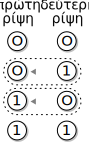
\includegraphics[scale=\scaling]{illustrations/coin.pdf}%
\captionof*{figure}{Όταν ρίχνουμε ένα νόμισμα δύο φορές υπάρχουν τέσσερα πιθανά ενδεχόμενα. Τα δύο από αυτά, όταν το αποτέλεσμα κάθε ρίψης είναι διαφορετικό, είναι \emph{ισοπίθανα}, ακόμα κι όταν το νόμισμα είναι μεροληπτικό. Η μέθοδος του von Neumann επαναλαμβάνει τη ρίψη δύο νομισμάτων μέχρι να προκύψει ένα από τα δύο ισοπίθανα ενδεχόμενα, και επιστρέφει το αποτέλεσμα που σημειώνεται με το βελάκι, προσομοιώνοντας έτσι ένα δίκαιο νόμισμα.}}
Ο Jon von Neumann %ήταν ένας διάσημος μαθηματικός με καθοριστική συμβολή (και) στην ανάπτυξη των πρώτων ηλεκτρονικών υπολογιστών.
σκέφτηκε έναν τρόπο να προσομοιώσει κανείς τη ρίψη ενός δίκαιου νομίσματος, ακόμα κι αν έχει στη διάθεσή του ένα μεροληπτικό νόμισμα. Η μέθοδος που πρότεινε είναι η εξής:
\begin{quote}
Ρίξε το μεροληπτικό νόμισμα δύο φορές. Αν το αποτέλεσμα σε κάθε ρίψη είναι διαφορετικό, τότε ανακοίνωσε το αποτέλεσμα της πρώτης ρίψης, αλλιώς επανάλαβε τη διαδικασία. 
\end{quote}
Το αποτέλεσμα αυτής της μεθόδου ισοδυναμεί με το αποτέλεσμα της ρίψης ενός δίκαιου νομίσματος. 
% Με ένα μεροληπτικό νόμισμα, η πιθανότητα να φέρει κανείς Κορώνα και μετά Γράμματα, είναι η ίδια με το να φέρει κανείς Γράμματα και μετά Κορώνα. Γι' αυτό το λόγο, το αποτέλεσμα που ανακοινώνεται με τη μέθοδο του von Neumannn αντιστοιχεί στη ρίψη ενός δίκαιου νομίσματος.

Να γράψετε συνάρτηση με όνομα \pyinline{flipFair}, η οποία θα μιμείται τη ρίψη ενός δίκαιου νομίσματος και θα επιστρέφει είτε το \pyinline{0}, είτε το \pyinline{1}. Η συνάρτηση θα πρέπει να χρησιμοποιεί τη μέθοδο του von Neumann: θα υπολογίζει το αποτέλεσμά της χρησιμοποιώντας ένα μεροληπτικό νόμισμα, δηλαδή καλώντας την συνάρτηση \pyinline{flipBiased}.

Να φτιάξετε ένα πρόγραμμα που ελέγχει αν οι συναρτήσεις \pyinline{flipBiased} και \pyinline{flipFair} λειτουργούν όπως θα περιμέναμε.
Για κάθε συνάρτηση, το πρόγραμμα θα πρέπει να την καλεί επαναληπτικά  και να υπολογίζει το ποσοστό των ρίψεων στις οποίες το αποτέλεσμα ήταν το \pyinline{0}. Αν η \pyinline{flipBiased} λειτουργεί σωστά, τότε το ποσοστό αυτό θα πρέπει να προσεγγίζει το \pyinline{p}. Αν η \pyinline{flipFair} λειτουργεί σωστά, τότε το ποσοστό αυτό θα πρέπει να προσεγγίζει το \pyinline{50}. 

\begin{note} 
Καλό θα ήταν ο ίδιος ο χρήστης να παρέχει την τιμή της παραμέτρου \pyinline{p} της \pyinline{flipBiased} και το πλήθος των επαναλήψεων. 
Έτσι θα μπορέσετε κι εσείς, ως χρήστες, να πειραματιστείτε εύκολα με διάφορες τιμές. Όπως ισχύει σε κάθε προσομοίωση, το πλήθος των επαναλήψεων πρέπει να είναι μεγάλο (π.χ. τουλάχιστον 10000), για να είναι το αποτέλεσμα του ελέγχου αξιόπιστο. 
% Χρησιμοποιήστε όποια τιμή θέλετε για την παράμετρο \pyinline{p} της \pyinline{flipBiased}, αρκεί αυτή να μην είναι κοντά στο \pyinline{50}. Επίσης, όπως ισχύει σε κάθε προσομοίωση, καλό θα ήταν το πλήθος των επαναλήψεων να είναι μεγάλο (π.χ. τουλάχιστον 10000), για να είναι το αποτέλεσμα αξιόπιστο.
\end{note}
\solutionlink{guess}{flip-biased.py}
\end{exercise}

% Παιχνίδι δύο παικτών παίκτη-υπολογιστή, μαντεύουν εναλλάξ. Κερδίζει αυτός που θα το βρει πρώτος. Αν ο παίκτης ξέρει την στρατηγική του υπολογιστή, μπορεί να μεγιστοποιήσει τον αριθμό των προσπαθειών...
%\begin{exercise}
%\solutionlink{guess}{guess-twoplayer.py}
%\end{exercise}

%%%%%%%%

\section*{}
%\vspace{4\parskip}
\hrulefill

%\begin{theory}{Τύποι Και Αναπαραστάσεις}
%\end{theory}

\begin{theory}{Αναζήτηση}
Όταν ψάχνουμε κάτι, όπως για παράδειγμα έναν μυστικό αριθμό, μιλάμε για \emph{αναζήτηση}. Η αναζήτηση είναι κάτι που κάνουμε πολύ συχνά, είτε μόνοι μας, είτε με τη βοήθεια υπολογιστών. Ψάχνουμε για ένα όνομα στον τηλεφωνικό κατάλογο ή για την επόμενη κίνηση σ' ένα επιτραπέζιο παιχνίδι. Συχνά η αναζήτηση δεν είναι καθόλου απλή υπόθεση. Μπορεί ο χώρος στον οποίο ψάχνουμε να είναι αχανής. Μπορεί να μην ξέρουμε τι ακριβώς ψάχνουμε ή πως πρέπει να το περιγράψουμε. Για παράδειγμα, η μηχανή αναζήτησης της Google προσπαθεί μέσα σε μερικά δέκατα του δευτερολέπτου να συγκεντρώσει και να ταξινομήσει τις διευθύνσεις των ιστοσελίδων που πιθανώς μας ενδιαφέρουν, βασισμένη κάθε φορά σε μερικές λέξεις-κλειδιά που της παρέχουμε. Οι βιολόγοι αναζητούν ακολουθίες αμινοξέων μέσα στον γενετικό μας κώδικα, παρέχοντας μόνο ένα γενικό πρότυπο γιατί μπορεί να υπάρχουν αποδεκτές παραλλαγές και μεταλλάξεις. Με δεδομένο πάντως το πόσο σημαντικό πρόβλημα είναι η αναζήτηση, είναι ευτυχές ότι πρόκειται για ένα πρόβλημα που λύνεται συνήθως πολύ αποδοτικά.
\end{theory}

\begin{theory}{Δυαδική Αναζήτηση}
Όταν αναζητούμε ένα αντικείμενο μέσα σε ένα σύνολο από \emph{ταξινομημένα} στοιχεία τότε το καλύτερο που μπορούμε να κάνουμε είναι να ψάξουμε ακριβώς στη μέση. Αν το μεσαίο στοιχείο δεν είναι αυτό που ψάχνουμε τότε (επειδή τα στοιχεία είναι ταξινομημένα) γνωρίζουμε προς τα που πρέπει να συνεχίσουμε την αναζήτηση, αποκλείουμε μεμιάς τα άλλα μισά στοιχεία που βρίσκονται προς την αντίθετη κατεύθυνση και εφαρμόζουμε την ίδια διαδικασία στα στοιχεία που απομένουν. Με τον τρόπο αυτό, είτε θα εντοπίσουμε κάποια στιγμή το στοιχείο που αναζητούμε, είτε θα εξαντληθούν τα στοιχεία και θα φτάσουμε στο συμπέρασμα ότι αυτό που ψάχνουμε δεν υπάρχει ανάμεσά τους. Αυτή η μέθοδος ονομάζεται δυαδική αναζήτηση και είναι ουσιαστικά η διαδικασία που ακολουθήσαμε στο τελευταίο βήμα του παραδείγματος για να εντοπίσουμε τον μυστικό αριθμό. 
% Θυμηθείτε ότι προϋπόθεση για την εφαρμογή της δυαδικής αναζήτησης είναι τα στοιχεία να είναι ταξινομημένα. Αν αυτό δεν ισχύει, το καλύτερο που μπορούμε να κάνουμε είναι να ελέγξουμε τα στοιχεία με την σειρά.
\end{theory}

\begin{theory}{Διαίρει και Βασίλευε}
Πρόκειται για μια στρατηγική επίλυσης προβλημάτων που στηρίζεται στον κατακερματισμό ενός προβλήματος σε μικρότερα υποπροβλήματα. Αυτά είναι συνήθως του ίδιου ή συναφούς τύπου με το αρχικό πρόβλημα και, στην καλύτερη περίπτωση, ίδιου μεγέθους μεταξύ τους. Τα υποπροβλήματα επιλύονται ξεχωριστά και, αν αυτό είναι απαραίτητο, οι λύσεις τους συνδυάζονται για να επιλυθεί το αρχικό πρόβλημα. Ουσιαστικά μια παρόμοια στρατηγική ακολουθούμε όταν το πρόβλημα που μας τίθεται είναι ο εντοπισμός του μυστικού αριθμού. Σε κάθε βήμα βρισκόμαστε αντιμέτωποι με το ίδιο πρόβλημα, αλλά τα όρια ανάμεσα στα οποία αναζητούμε τον αριθμό ολοένα και στενεύουν. Πολλοί σημαντικοί αλγόριθμοι στην Πληροφορική βασίζονται στη στρατηγική του διαίρει και βασίλευε.
% (Ο ορισμός ακολουθεί το βιβλίο \emph{Algorithmic Puzzles} του Levitin.)
\end{theory}

\hrulefill

\end{document}
